% Exam packages %
\documentclass[addpoints]{exam}
\usepackage[utf8]{inputenc}
\usepackage{multicol}
\setlength{\columnsep}{1cm}
\usepackage{nopageno}
\usepackage{graphicx}
\usepackage{amsmath}
\usepackage{tabu}
\usepackage{tikz}
\usepackage{wrapfig}
\graphicspath{{ images\ }}
% Chess notation package + English %
\usepackage{skak}
\usepackage[english]{babel}
% Formatting %
\pagestyle{headandfoot}
\firstpageheadrule
\firstpagefootrule
\runningheadrule
\firstpageheader{Name:}{\Large{\textbf{2017 Final Exam}}}{Block: \ \ \ }
\runningheader{Name:}{\large{\textbf{2017 Final Exam}}}{Block: \ \ \ }
\runningfootrule
\firstpagefooter{PreCalc Fun}{ Page \thepage\ of \numpages}{Ethan Moscot}
\runningfooter{PreCalc Fun}{ Page \thepage\ of \numpages}{Ethan Moscot}

\begin{document}
% Directions & Grading Info %
\begin{center}
\fbox{\fbox{\parbox{7in}{\centering
The content on this final exam is mostly placed in chronological order within each section, from Unit 1-Unit 8.
\newline Answer all non-multiple choice questions to the best of your ability in order to receive the greatest amount of credit.}}}
\end{center}
\begin{center}
This final exam has \numquestions\ questions (100 exam questions and 2 bonus questions), worth a total of \numpoints\ points in addition to \numbonuspoints\ bonus points.
Good luck!
\end{center}

% Multiple Choice section %
\section*{Multiple Choice}
    \begin{questions}
    \setcounter{question}{0}
    % Units 1 & 2 %
    \question[1] If a non-horizontal line has a slope of $\sin(\theta)$, it will be perpendicular to a line with slope...
    % (This problem was taken directly from a past test.)
    
    \begin{oneparchoices}
        \choice $\cos\theta$ 
        \choice $-\cos\theta$
        \choice $\csc\theta$
        \choice $-\csc\theta$
        \choice $-\sin\theta$
        \end{oneparchoices} \vspace{\stretch{1}} \answerline
    
    \question[1] Which quadrant is the angle $75^\circ$ in?

    \begin{oneparchoices}
        \choice QI 
        \choice QII
        \choice QIII
        \choice QIV
        \end{oneparchoices} \vspace{\stretch{1}} \answerline
        
    \question[1] In how many different ways can the letters in MISSISSIPPI be arranged?
    
    \begin{oneparchoices}
        \choice 7560
        \choice 34650
        \choice 75600
        \choice 151200
        \choice 302400
        \end{oneparchoices} \vspace{\stretch{1}} \answerline
        
    \question[1] Given the angle $92^\circ$, find the reference angle.
    
    \begin{oneparchoices}
        \choice $90^\circ$
        \choice $8^\circ$
        \choice $272^\circ$
        \choice $180^\circ$
        \choice $2^\circ$
        \end{oneparchoices} \vspace{\stretch{1}} \answerline
        
    % Unit 3 %
    
    \question[1] Choose the answer that best describes the transformation of $f(\frac{1}{3}x)$.
    
     \begin{oneparchoices}
        \choice vertical stretch
        \choice vertical compression
        \choice horizontal stretch
        \choice horizontal compression
        \end{oneparchoices} \vspace{\stretch{1}} \answerline
    
    \question[1] Choose the answer that best describes the transformation of $f(x+5)$.
    
    \begin{oneparchoices}
        \choice vertical stretch
        \choice vertical compression
        \choice horizontal stretch
        \choice horizontal translation
        \end{oneparchoices} \vspace{\stretch{1}} \answerline
    
    \question[1] Given $f(x) = x^2 - 8$ and $g(x) = -5 - x$, find $f(g(x))$.
    
    \begin{oneparchoices}
        \choice $x^2 + 10x + 17$
        \choice $-x^2 - 13$
        \choice $-x^2 + 3$
        \choice $x^2 - 10x + 3$
        \end{oneparchoices} \vspace{\stretch{1}} \answerline
    
    % Unit 4 %
    
    \question[1] Order the functions from the widest to narrowest graph, given $f(x) = \frac{1}{3}x^2$, $g(x) = -9x^2$ and $h(x) = \frac{-1}{2}x^2$.
    
    \begin{oneparchoices}
        \choice $f(x)$, $g(x)$ and $h(x)$
        \choice $h(x)$, $f(x)$ and $g(x)$
        \choice $f(x)$, $h(x)$ and $g(x)$
        \choice $g(x)$, $h(x)$ and $f(x)$
        \choice $g(x)$, $f(x)$ and $h(x)$
        \end{oneparchoices} \vspace{\stretch{1}} \answerline
        \newpage
    
    \question[1] What is the multiplicity of the zero $x = -4$ in $f(x) = (x+1)^2 (x+4)^3 (x-6)^5 (x-4)^6$?
    
    \begin{oneparchoices}
        \choice 2
        \choice 1
        \choice 3
        \choice 5
        \choice 6
        \end{oneparchoices} \vspace{\stretch{1}} \answerline
    
    \question[1] Given the point $(-3, -3)$, determine the sign of $tan(\theta)$.
    
    \begin{oneparchoices}
        \choice Positive
        \choice Negative
        \choice Neutral
        \choice QIV
        \choice None of the above
        \end{oneparchoices} \vspace{\stretch{1}} \answerline
    
    % Unit 5 %
    \question[1] The growth factor for $f(x) = \frac{5}{6}\cdot (4)^x$ is
    
    \begin{oneparchoices}
        \choice $\frac{6}{5}$ 
        \choice $\frac{1}{4}$
        \choice $\frac{5}{6}$
        \choice 5
        \choice 4
        \end{oneparchoices} \vspace{\stretch{1}} \answerline

    \question[1] What is the constant percentage decay rate of $P(t) = 2.609 \cdot 0.093^t$?
    
    \begin{oneparchoices}
        \choice 93\%
        \choice 0.093\%
        \choice 26.09\%
        \choice 90.7\%
        \choice 260.9\%
        \end{oneparchoices} \vspace{\stretch{1}} \answerline
    
    \question[1] What is the approximate value of the common log of 5?
    
    \begin{oneparchoices}
        \choice 0.69897
        \choice 1.60943
        \choice 5
        \choice 3.30103
        \choice Undefined
        \end{oneparchoices} \vspace{\stretch{1}} \answerline
    
    % Unit 6 %
    
    \question[1] The graph of $y = \csc(x)$ never intersects the graph of $y =$
    
    \begin{oneparchoices}
        \choice $x$
        \choice $x^2$
        \choice $\cos(x)$
        \choice $\csc(x)$
        \choice $\sin(x)$
        \end{oneparchoices} \vspace{\stretch{1}} \answerline
    
    \question[1] If $\theta$ is the smallest angle in a 3-4-5 triangle, then what is the $\cos(\theta)$?
    
    \begin{oneparchoices}
        \choice $\frac{3}{5}$
        \choice $\frac{5}{4}$
        \choice $\frac{4}{3}$
        \choice $\frac{3}{4}$
        \choice $\frac{4}{5}$
        \end{oneparchoices} \vspace{\stretch{1}} \answerline
    
    \question[1] A sinusoid with an amplitude of 3 has a minimum value of -2. Its maximum value is
    
    \begin{oneparchoices}
        \choice 10
        \choice 6
        \choice 4
        \choice 2
        \choice -2
        \end{oneparchoices} \vspace{\stretch{1}} \answerline
    
    % Unit 7 %
    
    \question[1] Simplify $\cos(-x)$
    
    \begin{oneparchoices}
        \choice $\sec x$
        \choice $\csc -x$
        \choice $-\cos x$
        \choice $\cos x$
        \choice $\cos \frac{1}{x}$
        \end{oneparchoices} \vspace{\stretch{1}} \answerline
    
    \question[1] A simpler expression for $(1 - \sin \theta)(1 + \sin \theta)$ is
    
    \begin{oneparchoices}
        \choice $\sin^2 \theta + \cos^2 \theta$
        \choice $\sin^2\theta$
        \choice $-\sin^2\theta$
        \choice $\cos^2\theta$
        \choice $1 - \sin^2 \theta$
        \end{oneparchoices} \vspace{\stretch{1}} \answerline
    
    \question[1] Write the expression $\sin 48^\circ \cos 15^\circ - \cos 48^\circ \sin 15^\circ$ as a single sine or cosine of an angle. 
    
    \begin{oneparchoices}
        \choice $\cos 63^\circ$
        \choice $\sin 63^\circ$
        \choice $\sin 15^\circ$
        \choice $\cos 15^\circ$
        \choice $\sin 33^\circ$
        \end{oneparchoices} \vspace{\stretch{1}} \answerline
    
    % Unit 8 %
    
    \question[1] Let \textbf{a} = $\big \langle 3, 4 \big \rangle\ $and \textbf{b} = $\big \langle -5, 6 \big \rangle\ $. Which of the following is equal to \textbf{a} - \textbf{b}?
    
    \begin{oneparchoices}
        \choice $\big \langle -1, -11 \big \rangle\ $
        \choice $\big \langle 8, -2 \big \rangle\ $
        \choice $\big \langle -2, 10 \big \rangle\ $
        \choice $\big \langle 3, 4 \big \rangle\ $- $\big \langle -5, 6 \big \rangle\ $
        \choice $\big \langle -15, 20 \big \rangle\ $
        \end{oneparchoices} \vspace{\stretch{1}} \answerline
    
    \question[1] Let \textbf{a} = $\big \langle 2, 4 \big \rangle\ $and \textbf{b} = $\big \langle 3, 5 \big \rangle\ $. Which of the following is equal to \textbf{a} \cdot \textbf{b}?

    \begin{oneparchoices}
        \choice 90
        \choice 23
        \choice 26
        \choice 120
        \choice $\big \langle 6, 20 \big \rangle\ $
        \end{oneparchoices} \vspace{\stretch{1}} \answerline
    
    \question[1] Which of the following gives the number of petals of the rose curve $r = 5\cos4\theta$?
    
    \begin{oneparchoices}
        \choice 2
        \choice 4
        \choice 6
        \choice 8
        \choice 10
        \end{oneparchoices} \vspace{\stretch{1}} \answerline
    
    \question[1] Let \textbf{a} = $\big \langle 1, 4 \big \rangle\ $and \textbf{b} = $\big \langle 2, 6 \big \rangle\ $. Find the component form of the vector given $3\textbf{b}$.
    
    \begin{oneparchoices}
        \choice $\big \langle 6, 18 \big \rangle\ $
        \choice $\big \langle 6, 8 \big \rangle\ $
        \choice $\big \langle 9b, 15b \big \rangle\ $
        \choice $\big \langle 6, 12 \big \rangle\ $
        \choice $\big \langle 6, 20 \big \rangle\ $
        \end{oneparchoices} \vspace{\stretch{1}} \answerline
    
    \question[1] Let \textbf{a} = $\big \langle 3, 7 \big \rangle\ $and \textbf{b} = $\big \langle 2, 9 \big \rangle\ $. Find the component form of the vector given $32\textbf{a}$.
    
    \begin{oneparchoices}
        \choice $\big \langle 48, 144 \big \rangle\ $
        \choice $\big \langle 96a, 224b \big \rangle\ $
        \choice $\big \langle 64, 169 \big \rangle\ $
        \choice $\big \langle 96, 160 \big \rangle\ $
        \choice $\big \langle 96, 224 \big \rangle\ $
        \end{oneparchoices} \vspace{\stretch{1}} \answerline
    
    \question[1] Let \textbf{a} = $\big \langle 1, 3 \big \rangle\ $and \textbf{b} = $\big \langle 4, 6 \big \rangle\ $. Find the component form of the vector given $3\textbf{a} - 4\textbf{b}$.
    
    \begin{oneparchoices}
        \choice $\big \langle 19, 33 \big \rangle\ $
        \choice $\big \langle -13, -15 \big \rangle\ $
        \choice $\big \langle 12, 40 \big \rangle\ $
        \choice $\big \langle 12a, 40b \big \rangle\ $
        \choice $\big \langle 27, 384 \big \rangle\ $
        \end{oneparchoices} \vspace{\stretch{1}} \answerline
    \end{questions}
    
\newpage
% Short Answer section %
\section*{Short Answer (Open Ended)}
    \begin{questions}
    \setcounter{question}{25}
    % Units 1 & 2 %
    \question[1] Use this table of frequencies for colors of Skittles in a bag to solve the following problems.
    \begin{center}
            \begin{tabular}{ |c|c|c|c|c|c| } 
            \hline
            red & orange & yellow & green & blue & brown \\
            \hline
            0.1 & 0.2 & 0.1 & 0.2 & 0.1 & 0.3 \\
            \hline
            \end{tabular} 
        \end{center}
        
        \begin{parts}
            \part What is the probability of selecting one orange or green Skittle out of the bag? \vspace{\stretch{1}}
    
            \part What is the probability of \textbf{not} selecting one yellow or one blue Skittle out of the bag? \vspace{\stretch{1}}
    
            \part Suppose there are two bags of Skittles. What is the probability of picking one brown from one bag and one red from the other bag?  \vspace{\stretch{1}} \end{parts}
    
    \question[1] You are rolling two dice and are taking the sum of the numbers rolled. 
        \begin{parts}
            \part State the probability of rolling a 6 or 11. \vspace{\stretch{1}}
    
            \part State the probability of rolling a number divisible by 2. \vspace{\stretch{1}}
            
            \part State the probability of rolling a double-digit number. \vspace{\stretch{1}} \end{parts} 
    \newpage
    \question[1] Given $129^\circ$, express one positive coterminal angle and one negative coterminal angle.
    \vspace{\stretch{1}}
    
    \question[1] From among 8 projects for consideration, the mayor must put together a prioritized list of 3 projects to submit to the city council for funding. How many lists can be formed? 
    \vspace{\stretch{1}}
    
    \question[1] Convert $\frac{3\pi}{2}$ from radians to degrees \textbf{AND} state which quadrant the angle is in. The answer should be simplified to the tenth. \vspace{\stretch{1}} 
    
    % Unit 3 %
    
    \question[1] Determine the domain of $f(x) = \frac{5}{x^2 - 4}$ algebraically. \vspace{\stretch{1}}
    
    \question[1] Determine the domain of $f(x) = \sqrt{x^2 + 13} $ algebraically. \vspace{\stretch{1}}
    
    \question[1] Given $f(x) = 3x - 5$ and $g(x) = x - 2$, find $f(g(x))$. \vspace{\stretch{1}}
    
    \question[1] Given $f(x) = x^2 + 1$ and $g(x) = \frac{1}{x^2 + 4}$, find $f(g(x))$. \vspace{\stretch{1}}
         
    % Unit 4 %
    
    \question[1] Determine the slant asymptote of $f(x) = \frac{x^2 - 6x + 7}{x + 5}$ algebraically. \vspace{\stretch{1}}
    
    \question[1] Determine the slant asymptote of $f(x) = \frac{3x^3 - 2x}{-2x^2 + 4}$ algebraically. \vspace{\stretch{1}}
    
    \newpage
    \question[1] Solve the equation. $\frac{4x}{x - 1} + \frac{6}{x + 2} = \frac{24}{x^2 + x - 2}$
    \vspace{\stretch{1}}
    
    % Unit 5 %
    
    \question[1] Expand the following (rewrite as an expanded logarithm): $\ln(7xy)$. \vspace{\stretch{1}}
    
    \question[1] Condense the following (rewrite as a single, condensed logarithm): $\log 12 + \log x + \log y$. \vspace{\stretch{1}}
    
    \question[1] The number B of a flesh-eating bacteria in a petri dish culture after t hours is given by $$B = 68e^{0.867t}$$
        \begin{parts}
            \part What is the initial amount of bacteria present? \vspace{\stretch{1}}
    
            \part What is the rate that the bacteria are increasing at? \vspace{\stretch{1}}
            
            \part How many bacteria are present after 8 $\frac{1}{2}$ hours? \vspace{\stretch{1}} 
            
            \part How many bacteria are present after 3 days? \vspace{\stretch{1}} \end{parts}
     
    % Unit 6 %
    
    \question[1] Find the exact value of $\sin^{-1} (\frac{\sqrt{2}}{2})$ using the unit circle. \vspace{\stretch{1}}
    
    \question[1] Find the exact value of $\cos^{-1} (\frac{1}{2})$ using the unit circle. \vspace{\stretch{1}}
    
    \question[1] Using the unit circle, find the exact value of $\cos(150^\circ)$. \vspace{\stretch{1}}
    
    \question[1] Using the unit circle, find the exact value of $\csc(60^\circ)$. \vspace{\stretch{1}}
    
    \newpage
    \question[1] State the amplitude, period, phase shift and vertical shift of $$y = 7\cos(x - \pi) + 6$$. 
    \newline
    Amplitude: \line(1,0){40} \\
    \newline
    Period: \line(1,0){40} \\
    \newline
    Phase Shift: \line(1,0){40} \\
    \newline
    Vertical Shift: \line(1,0){40}
    \vspace{\stretch{0.5}}
 
    % Unit 7 %
    
    \question[1] Simplify $\cot\theta\csc\theta$. \vspace{\stretch{1}}
    
    \question[1] Verify that $\cos x + \sin x + \tan x$ is $\sec x$ \vspace{\stretch{1}}
    % (This problem was taken directly from a past test.)
    
    \question[1] Verify that $\frac{1}{1 - \sin\theta} + \frac{1}{1 + \sin\theta}$ is $2\sec^2\theta$ \vspace{\stretch{1}}
    % (This problem was taken directly from a past test.)
    
    \question[1] Find all values of $x$ in the interval $[0, 2\pi)$ that solves $2\cos x + 2 = 0$. The answer can be provided in either radians or degrees. \vspace{\stretch{1}}
    
    \newpage
    \question[1] Solve $\triangle ABC$ given that $\angle A = 60^\circ, b = 15$ and $c = 22$. \vspace{\stretch{2}}
    
    \question[1] Solve $\triangle ABC$ given that $a = 20, b = 30$ and $\angle B = 140^\circ$. \vspace{\stretch{2}}
    
    % Unit 8 %
    
    \question[1] Solve the non-linear system: $$x^2 + y = 6$$
    $$x + y = 14$$ \vspace{\stretch{1}}
    
    \question[1] Convert $y = 2x + 1$ from rectangular to polar form. \vspace{\stretch{1}}
    
    \question[1] Convert $r(2\cos\theta + \sin\theta) = 4$ from polar to rectangular form. \vspace{\stretch{1}}
    
    \question[1] Perform the following matrix operation:
    \begin{bmatrix} 
    1 & -7 \\
    0 & 3 \\
    5 & -10
    \end{bmatrix}
    $+$
    \begin{bmatrix} 
    11 & 17 \\
    -12 & 8 \\
    4 & 9
    \end{bmatrix}
    \vspace{\stretch{1}}
    \end{questions}
    
\newpage
% Word Problems section %
\section*{Word Problems}
    \begin{questions}
    \setcounter{question}{55}
    % Units 1 & 2 %
    \question[1] You are about to go base jumping and are second guessing if the cliff you are standing on is tall enough. You ask your friend to help you measure the height so she goes down to the bottom of the cliff to help you measure the height. She starts at the base of the cliff and walks out 100 meters. You measure an angle of depression of $44^\circ$ from the horizon to her. When you base jump you you prefer to be at least 100 meters above the ground to give yourself time to safely deploy your parachute. Should you attempt this base jump? Give a mathematical reason for your decision.
    %(This problem was taken directly from a past test.)

        \vspace{0.5cm}
        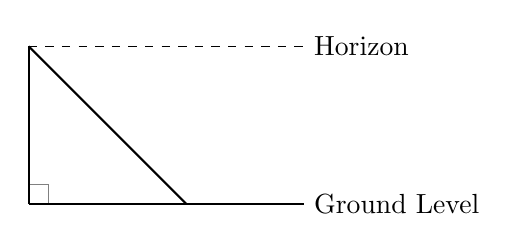
\begin{tikzpicture}[scale=.5]
        \draw [gray] (0,0) rectangle (0.5,0.5);
        \draw[black, thick] (0,0) -- (0,4);
        \draw[black, thick] (0,0) -- (7,0);
        \draw[black, thick] (0,4) -- (4,0);
        \draw[dashed]  (0,4) -- (7,4);
        \node[right] at (7,0) {Ground Level};
        \node[right] at (7,4) {Horizon};
        \end{tikzpicture} \vspace{\stretch{1}}
        
    % Unit 3 %
    
    \question[1] You are given an 8.5in $\times$ 11.5in piece of paper. After using it, you decide to cut out a square of the same size from each corner. After you cut out the squares, you fold the paper into an open box.
    %(This problem has been copied directly from a previous test.)
        \begin{parts}
            \part Draw a diagram for the piece of paper and for the open top box. Include variables and known values. \vspace{\stretch{2}}
    
            \part What is the interval for plausible $x$ values, where x is the side length of the square you cut out? \vspace{\stretch{2}}
            
            \part What is the equation for volume, with respect to $x$? \vspace{\stretch{2}} 
            
            \part What is the $x$ value that maximizes the volume? \vspace{\stretch{2}} 
            
            \part What is the maximum volume?
            \vspace{\stretch{2}}
            \end{parts}
    
    \newpage
    % Unit 4 %
    
    \question[1] How much pure acid must be added to 75 mL of a 50\% acid solution in order to produce a mixture that is 80\% acid? \vspace{\stretch{1}}
    
    \question[1] Find the dimensions of the rectangle with minimum perimeter if its area is 400 square feet. Find this least perimeter. 
    \vspace{\stretch{1}}
    
    % Unit 5 %
    
    \question[1] Given $A = Pe^{rt}$, suppose Rob invests $\$150$ at a $12\%$ interest rate compounded continuously. Find the value of his investment at the end of 6 years. 
    \vspace{\stretch{1}}
    
    \question[1] Assume Harper invests \$1200 at an 8\% interest rate compounded quarterly. 
    \newline Given $A = P(1 + \frac{r}{n})^{(nt)}$, how much money will she have in 3 years?
    \vspace{\stretch{1}}
    
    \question[1] Suppose Jim invests \$800 at an 9\% interest rate compounded quarterly. 
    \newline Given $A = P(1 + \frac{r}{n})^{(nt)}$, how much will he have \textbf{earned} in 4 years? \vspace{\stretch{1}}
    
    \question[1] Warren Buffett invested \$20,000 twice into two separate bank accounts (his total investment was \$40,000). One account pays 2\% in interest monthly and the other pays 6\% in interest annually. Given $A = P(1 + \frac{r}{n})^{(nt)}$, determine how much money, in total, he \textbf{earned} over the course of two years. \vspace{\stretch{1}}
    
    % Unit 6 %
    
    \question[1] The angle of depression from the top of a lighthouse 250ft above sea level to a sailboat is $12^\circ$. How far is the boat from the base of the lighthouse? \vspace{\stretch{2}}

    \question[1] A wire stretches from the top of a tower to the ground 40ft away from the base of the tower. The wire makes an angle of $70^\circ$ with the ground. Find the height of the tower and the length of the wire. 
    \vspace{\stretch{2}}
    
    \newpage
    % Unit 7 %
    
    \question[1] Two points, $A$ and $B$, are on the same side of a canyon and are 70ft apart. A hiker is located across the rim at point $C$. A surveyor determines that $\angle BAC$ is $60^\circ$ and $\angle ABC$ is $65^\circ$.
    \begin{parts}
        \part Sketch a diagram of this situation.
        \vspace{\stretch{2}}
        
        \part What is the distance between the hiker and point $A$? \vspace{\stretch{2}}
        \end{parts}
     
    \question[1] A boat leaves Miami and heads due east for 35km. At the same time, a second boat also travels from Miami for 25km. The two boats are 15.2km apart when they reach their final destination.
        \begin{parts} 
        \part Sketch a diagram of this situation. \vspace{\stretch{2}}
    
        \part What was the angle between the two boats when they left Kingston? \vspace{\stretch{2}}
        \end{parts} 
        
    % Unit 8 %
    
    \question[1] A ship is heading due north at 16mph. The current is flowing southwest at 5mph. 
        \begin{parts}
            \part Sketch a diagram of this scenario.
            \vspace{\stretch{2}}
    
            \part Find the actual bearing and speed of the ship. \vspace{\stretch{2}} \end{parts}
    
    \newpage
    \question[1] The admission fee at the Iowa state fair is \$1.50 for children and \$4.00 for adults. On a certain day, 2200 people enter the fair and \$5,050 is collected. How many children and how many adults attended? \vspace{\stretch{1}}
    
    \question[1] At a movie premiere, 351 tickets were sold. The cost for child admission was \$1.50 per ticket and the cost for adult admission was \$2.00. What was the total price of the adult tickets? \vspace{\stretch{1}} 
    
    \question[1] An exam worth 145 points contains 50 questions. Some of the questions are worth two points and some are worth five points. How many two point questions are on the test? How many five point questions are on the test? \vspace{\stretch{1}}
    \end{questions}
    
\newpage
% Graphing section %
\section*{Graphing}
    \begin{questions}
    \setcounter{question}{71}
    % Units 1 & 2 %
    \question[1] Given an angle in standard position with a terminal ray that passes through the point $(4,8)$, find the values of the six trigonometric functions. Graph this and label the point and the angle.

        \begin{left} 
        \begin{tikzpicture}[scale=1.3]
        \draw[gray] (-1.5,0) -- (1.5,0);
        \draw[gray] (0,1.5) -- (0,-1.5);
        \end{tikzpicture} 
        \end{left} \vspace{\stretch{0.5}}
        
    \question[1] Given an angle in standard position with a terminal ray that passes through the point $(-2,-5)$, find the values of the six trigonometric functions. Graph this and label the point and the angle.

        \begin{left} 
        \begin{tikzpicture}[scale=1.3]
        \draw[gray] (-1.5,0) -- (1.5,0);
        \draw[gray] (0,1.5) -- (0,-1.5);
        \end{tikzpicture} 
        \end{left} \vspace{\stretch{0.5}}
    
    % Unit 3 %
    
    \question[1] Sketch the graph of $f(x) = (x-3)^2 + 4$ and state its domain, range and parent function.
    
        \begin{left} 
        \begin{tikzpicture}[scale=1.3]
        \draw[gray] (-1.5,0) -- (1.5,0);
        \draw[gray] (0,1.5) -- (0,-1.5);
        \end{tikzpicture} 
        \end{left}
        
    Domain: \line(1,0){40} \\
    \newline
    Range: \line(1,0){40} \\
    \newline
    Parent Function: \line(1,0){40} \\
    \vspace{\stretch{0.5}}
    
    \newpage
    \question[1] Sketch the graph of $f(x) = -3|x+1| - 2$ and state its domain, range and parent function.
    
        \begin{left} 
        \begin{tikzpicture}[scale=1.3]
        \draw[gray] (-1.5,0) -- (1.5,0);
        \draw[gray] (0,1.5) -- (0,-1.5);
        \end{tikzpicture} 
        \end{left}
        
    Domain: \line(1,0){40} \\
    \newline
    Range: \line(1,0){40} \\
    \newline
    Parent Function: \line(1,0){40} \\
    \vspace{\stretch{0.5}}
    
    \question[1] Sketch the graph of $f(x) = \frac{3}{x - 4}$ and state its domain, range and parent function.
    
        \begin{left} 
        \begin{tikzpicture}[scale=1.3]
        \draw[gray] (-1.5,0) -- (1.5,0);
        \draw[gray] (0,1.5) -- (0,-1.5);
        \end{tikzpicture} 
        \end{left}
        
    Domain: \line(1,0){40} \\
    \newline
    Range: \line(1,0){40} \\
    \newline
    Parent Function: \line(1,0){40} \\
    \vspace{\stretch{0.5}}
    
    \question[1] Sketch the graph of the rational function $\frac{x}{x^2 - 4}$ and find its end behavior and vertical asymptote(s).
    
        \begin{left} 
        \begin{tikzpicture}[scale=1.3]
        \draw[gray] (-1.5,0) -- (1.5,0);
        \draw[gray] (0,1.5) -- (0,-1.5);
        \end{tikzpicture} 
        \end{left}
    
    $\lim_{x\to\infty} f(x)$ =
    \newline    
    $\lim_{x\to-\infty} f(x)$ =
    \newline
    Vertical Asymptote(s): \line(1,0){40} \\
    \vspace{\stretch{0.5}}
    
    \question[1] Sketch the graph of the rational function $\frac{2x - 2}{x - 4}$ and find its end behavior and vertical asymptote(s).
    
        \begin{left} 
        \begin{tikzpicture}[scale=1.3]
        \draw[gray] (-1.5,0) -- (1.5,0);
        \draw[gray] (0,1.5) -- (0,-1.5);
        \end{tikzpicture} 
        \end{left}
    
    $\lim_{x\to\infty} f(x)$ =
    \newline
    $\lim_{x\to-\infty} f(x)$ =
    \newline
    Vertical Asymptote(s): \line(1,0){40} \\
    \vspace{\stretch{0.5}}
    
    \question[1] Sketch the graph of the rational function $\frac{x^3}{x^2 - 16}$ and find its end behavior and vertical asymptote(s).
    
        \begin{left} 
        \begin{tikzpicture}[scale=1.3]
        \draw[gray] (-1.5,0) -- (1.5,0);
        \draw[gray] (0,1.5) -- (0,-1.5);
        \end{tikzpicture} 
        \end{left}
        
    $\lim_{x\to\infty} f(x)$ =
    \newline
    $\lim_{x\to-\infty} f(x)$ =
    \newline
    Vertical Asymptote(s): \line(1,0){40} \\
    \vspace{\stretch{0.5}}
   
    \question[1] Sketch the graph of the rational function $\frac{3x - 3}{x - 5}$ and find its end behavior and vertical asymptote(s).
    
        \begin{left} 
        \begin{tikzpicture}[scale=1.3]
        \draw[gray] (-1.5,0) -- (1.5,0);
        \draw[gray] (0,1.5) -- (0,-1.5);
        \end{tikzpicture} 
        \end{left}
        
    $\lim_{x\to\infty} f(x)$ =
    \newline
    $\lim_{x\to-\infty} f(x)$ =
    \newline
    Vertical Asymptote(s): \line(1,0){40} \\
    \vspace{\stretch{0.5}}
    
    \newpage
    % Unit 4 %
    
    \question[1] Sketch the graph of the function $f(x) = \frac{x^2 - 5}{x^2 - 4}$ and state the vertical and/or horizontal asymptote(s), slant asymptote(s), domain, range and end behavior.
    
        \begin{left} 
        \begin{tikzpicture}[scale=1.3]
        \draw[gray] (-1.5,0) -- (1.5,0);
        \draw[gray] (0,1.5) -- (0,-1.5);
        \end{tikzpicture} 
        \end{left}
    
    Vertical Asymptote(s): \line(1,0){40} \\
    \newline
    Horizontal Asymptote(s): \line(1,0){40} \\
    \newline
    Slant Asymptote(s): \line(1,0){40} \\
    \newline
    Domain: \line(1,0){40} \\
    \newline
    Range: \line(1,0){40} \\
    \newline
    $\lim_{x\to\infty} f(x)$: \line(1,0){40} \\
    \newline
    $\lim_{x\to-\infty} f(x)$: \line(1,0){40} \\
    \vspace{\stretch{0.5}}
    
    \question[1] Sketch the graph of the function $f(x) = \frac{-4}{x^2-8x+3}$ and state the vertical and/or horizontal asymptote(s), slant asymptote(s), domain, range and end behavior.
    
        \begin{left} 
        \begin{tikzpicture}[scale=1.3]
        \draw[gray] (-1.5,0) -- (1.5,0);
        \draw[gray] (0,1.5) -- (0,-1.5);
        \end{tikzpicture} 
        \end{left}
    
    Vertical Asymptote(s): \line(1,0){40} \\
    \newline
    Horizontal Asymptote(s): \line(1,0){40} \\
    \newline
    Slant Asymptote(s): \line(1,0){40} \\
    \newline
    Domain: \line(1,0){40} \\
    \newline
    Range: \line(1,0){40} \\
    \newline
    $\lim_{x\to\infty} f(x)$: \line(1,0){40} \\
    \newline
    $\lim_{x\to-\infty} f(x)$: \line(1,0){40} \\
    \vspace{\stretch{0.5}}
    
    \newpage
    \question[1] Sketch the graph of the function $f(x) = \frac{x+4}{x+3}$ and state the vertical and/or horizontal asymptote(s), slant asymptote(s), domain, range and end behavior.
    
        \begin{left} 
        \begin{tikzpicture}[scale=1.3]
        \draw[gray] (-1.5,0) -- (1.5,0);
        \draw[gray] (0,1.5) -- (0,-1.5);
        \end{tikzpicture} 
        \end{left}
    
    Vertical Asymptote(s): \line(1,0){40} \\
    \newline
    Horizontal Asymptote(s): \line(1,0){40} \\
    \newline
    Slant Asymptote(s): \line(1,0){40} \\
    \newline
    Domain: \line(1,0){40} \\
    \newline
    Range: \line(1,0){40} \\
    \newline
    $\lim_{x\to\infty} f(x)$: \line(1,0){40} \\
    \newline
    $\lim_{x\to-\infty} f(x)$: \line(1,0){40} \\
    \vspace{\stretch{0.5}}
    
    \question[1] Sketch the graph of the function $f(x) = \frac{5}{x^2 - 16}$ and state the vertical and/or horizontal asymptote(s), slant asymptote(s), domain, range and end behavior.
    
        \begin{left} 
        \begin{tikzpicture}[scale=1.3]
        \draw[gray] (-1.5,0) -- (1.5,0);
        \draw[gray] (0,1.5) -- (0,-1.5);
        \end{tikzpicture} 
        \end{left}
    
    Vertical Asymptote(s): \line(1,0){40} \\
    \newline
    Horizontal Asymptote(s): \line(1,0){40} \\
    \newline
    Slant Asymptote(s): \line(1,0){40} \\
    \newline
    Domain: \line(1,0){40} \\
    \newline
    Range: \line(1,0){40} \\
    \newline
    $\lim_{x\to\infty} f(x)$: \line(1,0){40} \\
    \newline
    $\lim_{x\to-\infty} f(x)$: \line(1,0){40} \\
    \vspace{\stretch{0.5}}
    
    \newpage
    % Unit 5 %
    
    \question[1] Given the function $f(x) = e^x + 5$, draw a sketch, state the vertical asymptote (as $x$ =) or horizontal asymptote (as $y$ =), domain, range and end behavior.
    
        \begin{left} 
        \begin{tikzpicture}[scale=1.3]
        \draw[gray] (-1.5,0) -- (1.5,0);
        \draw[gray] (0,1.5) -- (0,-1.5);
        \end{tikzpicture} 
        \end{left}
    
    Vertical Asymptote/Horizontal Asymptote: \line(1,0){40} \\
    \newline
    Domain: \line(1,0){40} \\
    \newline
    Range: \line(1,0){40} \\
    \newline
    $\lim_{x\to\infty} f(x)$: \line(1,0){40} \\
    \newline
    $\lim_{x\to-\infty} f(x)$: \line(1,0){40} \\
    \vspace{\stretch{0.5}}
    
    \question[1] Given the function $f(x) = 4^{x+5}$, draw a sketch, state the vertical asymptote (as $x$ =) or horizontal asymptote (as $y$ =), domain, range and end behavior.
    
        \begin{left} 
        \begin{tikzpicture}[scale=1.3]
        \draw[gray] (-1.5,0) -- (1.5,0);
        \draw[gray] (0,1.5) -- (0,-1.5);
        \end{tikzpicture} 
        \end{left}
    
    Vertical Asymptote/Horizontal Asymptote: \line(1,0){40} \\
    \newline
    Domain: \line(1,0){40} \\
    \newline
    Range: \line(1,0){40} \\
    \newline
    $\lim_{x\to\infty} f(x)$: \line(1,0){40} \\
    \newline
    $\lim_{x\to-\infty} f(x)$: \line(1,0){40} \\
    \vspace{\stretch{0.5}}
    
    \newpage
    \question[1] Given the function $f(x) = (\frac{3}{4})^x + 4$, draw a sketch, state the vertical asymptote (as $x$ =) or horizontal asymptote (as $y$ =), domain, range and end behavior.
    
        \begin{left} 
        \begin{tikzpicture}[scale=1.3]
        \draw[gray] (-1.5,0) -- (1.5,0);
        \draw[gray] (0,1.5) -- (0,-1.5);
        \end{tikzpicture} 
        \end{left}
    
    Vertical Asymptote/Horizontal Asymptote: \line(1,0){40} \\
    \newline
    Domain: \line(1,0){40} \\
    \newline
    Range: \line(1,0){40} \\
    \newline
    $\lim_{x\to\infty} f(x)$: \line(1,0){40} \\
    \newline
    $\lim_{x\to-\infty} f(x)$: \line(1,0){40} \\
    \vspace{\stretch{0.5}}
    
    \question[1] Given the function $f(x) = \log (x-2) + 1$, sketch a graph and state the vertical and horizontal asymptote(s), slant asymptote(s), domain, range and end behavior.
    
        \begin{left} 
        \begin{tikzpicture}[scale=1.3]
        \draw[gray] (-1.5,0) -- (1.5,0);
        \draw[gray] (0,1.5) -- (0,-1.5);
        \end{tikzpicture} 
        \end{left}
    
    Vertical Asymptote(s): \line(1,0){40} \\
    \newline
    Horizontal Asymptote(s): \line(1,0){40} \\
    \newline
    Slant Asymptote(s): \line(1,0){40} \\
    \newline
    Domain: \line(1,0){40} \\
    \newline
    Range: \line(1,0){40} \\
    \newline
    $\lim_{x\to\infty} f(x)$: \line(1,0){40} \\
    \newline
    $\lim_{x\to-\infty} f(x)$: \line(1,0){40} \\
    \vspace{\stretch{0.5}}
    
    \newpage
    \question[1] Given the function $f(x) = \ln(x) + 3$, sketch a graph and state the vertical and horizontal asymptote(s), slant asymptote(s), domain, range and end behavior.
    
        \begin{left} 
        \begin{tikzpicture}[scale=1.3]
        \draw[gray] (-1.5,0) -- (1.5,0);
        \draw[gray] (0,1.5) -- (0,-1.5);
        \end{tikzpicture} 
        \end{left}
    
    Vertical Asymptote(s): \line(1,0){40} \\
    \newline
    Horizontal Asymptote(s): \line(1,0){40} \\
    \newline
    Slant Asymptote(s): \line(1,0){40} \\
    \newline
    Domain: \line(1,0){40} \\
    \newline
    Range: \line(1,0){40} \\
    \newline
    $\lim_{x\to\infty} f(x)$: \line(1,0){40} \\
    \newline
    $\lim_{x\to-\infty} f(x)$: \line(1,0){40} \\
    \vspace{\stretch{0.5}}
    
    \question[1] Given the function $f(x) = 3\log(x-6)$, sketch a graph and state the vertical and horizontal asymptote(s), slant asymptote(s), domain, range and end behavior.
    
        \begin{left} 
        \begin{tikzpicture}[scale=1.3]
        \draw[gray] (-1.5,0) -- (1.5,0);
        \draw[gray] (0,1.5) -- (0,-1.5);
        \end{tikzpicture} 
        \end{left}
    
    Vertical Asymptote(s): \line(1,0){40} \\
    \newline
    Horizontal Asymptote(s): \line(1,0){40} \\
    \newline
    Slant Asymptote(s): \line(1,0){40} \\
    \newline
    Domain: \line(1,0){40} \\
    \newline
    Range: \line(1,0){40} \\
    \newline
    $\lim_{x\to\infty} f(x)$: \line(1,0){40} \\
    \newline
    $\lim_{x\to-\infty} f(x)$: \line(1,0){40} \\
    \vspace{\stretch{0.5}}
    
    \newpage
    % Unit 6 %
    
    \question[1] Graph $r = 4\sin(\theta) + 3$
    
        \begin{left} 
        \begin{tikzpicture}[scale=1.3]
        \draw[gray] (-1.5,0) -- (1.5,0);
        \draw[gray] (0,1.5) -- (0,-1.5);
        \end{tikzpicture} 
        \end{left}
    
    Range: \line(1,0){40} \\
    \newline
    Domain: \line(1,0){40} \\
    \newline
    Period: \line(1,0){40} \\
    \vspace{\stretch{0.5}}
    
    \question[1] Graph $r = 5\csc(\theta)- 4$
    
        \begin{left} 
        \begin{tikzpicture}[scale=1.3]
        \draw[gray] (-1.5,0) -- (1.5,0);
        \draw[gray] (0,1.5) -- (0,-1.5);
        \end{tikzpicture} 
        \end{left}
    
    Range: \line(1,0){40} \\
    \newline
    Period: \line(1,0){40} \\
    \vspace{\stretch{0.5}}
    
    \question[1] Graph $r = \sec(\theta + \frac{\pi}{4})+3$
    
        \begin{left} 
        \begin{tikzpicture}[scale=1.3]
        \draw[gray] (-1.5,0) -- (1.5,0);
        \draw[gray] (0,1.5) -- (0,-1.5);
        \end{tikzpicture} 
        \end{left}
    
    Range: \line(1,0){40} \\
    \newline
    Period: \line(1,0){40} \\
    \vspace{\stretch{0.5}}
    
    \newpage
    \question[1] Graph $r = 5(\sin(\theta))^2$
    
        \begin{left} 
        \begin{tikzpicture}[scale=1.3]
        \draw[gray] (-1.5,0) -- (1.5,0);
        \draw[gray] (0,1.5) -- (0,-1.5);
        \end{tikzpicture} 
        \end{left}
    
    Amplitude: \line(1,0){40} \\
    \newline
    Domain: \line(1,0){40} \\
    \newline
    Range: \line(1,0){40} \\
    \newline
    Period: \line(1,0){40} \\
    \vspace{\stretch{0.5}}
    
    % Unit 7: N/A %   
    % Unit 8 %
    
    \question[1] Sketch the function $r = 4\cos 2\theta$ and analyze the graph of the polar curve.
    
        \begin{left} 
        \begin{tikzpicture}[scale=1.3]
        \draw[gray] (-1.5,0) -- (1.5,0);
        \draw[gray] (0,1.5) -- (0,-1.5);
        \end{tikzpicture} 
        \end{left}
    
    Continuous: \line(1,0){40} \\
    \newline
    Symmetric: \line(1,0){40} \\
    \newline
    Domain: \line(1,0){40} \\
    \newline
    Range: \line(1,0){40} \\
    \vspace{\stretch{0.5}}
    
    \newpage
    \question[1] Sketch the function $r = 5 + \sin\theta$
    
        \begin{left} 
        \begin{tikzpicture}[scale=1.3]
        \draw[gray] (-1.5,0) -- (1.5,0);
        \draw[gray] (0,1.5) -- (0,-1.5);
        \end{tikzpicture} 
        \end{left}
    
    Continuous: \line(1,0){40} \\
    \newline
    Symmetric: \line(1,0){40} \\
    \newline
    Domain: \line(1,0){40} \\
    \newline
    Range: \line(1,0){40} \\
    \vspace{\stretch{0.5}}
    
    \question[1] Sketch the function $r = 7\cos3\theta$ and analyze the graph of the polar curve.
    
        \begin{left} 
        \begin{tikzpicture}[scale=1.3]
        \draw[gray] (-1.5,0) -- (1.5,0);
        \draw[gray] (0,1.5) -- (0,-1.5);
        \end{tikzpicture} 
        \end{left}
    
    Continuous: \line(1,0){40} \\
    \newline
    Symmetric: \line(1,0){40} \\
    \newline
    Domain: \line(1,0){40} \\
    \newline
    Range: \line(1,0){40} \\
    \vspace{\stretch{0.5}}
    
    \newpage
    \question[1] Sketch the function $r = 4\cos2\theta$ and analyze the graph of the polar curve.
    
        \begin{left} 
        \begin{tikzpicture}[scale=1.3]
        \draw[gray] (-1.5,0) -- (1.5,0);
        \draw[gray] (0,1.5) -- (0,-1.5);
        \end{tikzpicture} 
        \end{left}
    
    Continuous: \line(1,0){40} \\
    \newline
    Symmetric: \line(1,0){40} \\
    \newline
    Domain: \line(1,0){40} \\
    \newline
    Range: \line(1,0){40} \\
    \vspace{\stretch{0.5}}
    
    \question[1] Sketch the function $r = 8\cos4\theta$ and analyze the graph of the polar curve.
    
        \begin{left} 
        \begin{tikzpicture}[scale=1.3]
        \draw[gray] (-1.5,0) -- (1.5,0);
        \draw[gray] (0,1.5) -- (0,-1.5);
        \end{tikzpicture} 
        \end{left}
    
    Continuous: \line(1,0){40} \\
    \newline
    Symmetric: \line(1,0){40} \\
    \newline
    Domain: \line(1,0){40} \\
    \newline
    Range: \line(1,0){40} \\
    \vspace{\stretch{0.5}}
    
    \newpage
    \question[1] Sketch the function $r = 5\cos2\theta$ and analyze the graph of the polar curve.
    
        \begin{left} 
        \begin{tikzpicture}[scale=1.3]
        \draw[gray] (-1.5,0) -- (1.5,0);
        \draw[gray] (0,1.5) -- (0,-1.5);
        \end{tikzpicture} 
        \end{left}
    
    Continuous: \line(1,0){40} \\
    \newline
    Symmetric: \line(1,0){40} \\
    \newline
    Domain: \line(1,0){40} \\
    \newline
    Range: \line(1,0){40} \\
    \vspace{\stretch{0.5}}
    \end{questions}
    
\newpage
% Extra Credit section %
\section*{Extra Credit}
    \begin{questions}
    \setcounter{question}{100}
   
    \bonusquestion[10] Find checkmate in one move. Assume it is white's move and there is only one acceptable solution. \newline
    \newgame
    \fenboard{1Bb3BN/R2Pk2r/1Q5B/4q2R/2bN4/4Q1BK/1p6/1bq1R1rb w - - 0 20}
    \showboard
    
    \bonusquestion[3] Who founded the Cartesian coordinate system?
    \end{questions}   
\newpage
\section*{Formulas and Equations}
$a^2 = b^2 + c^2 -2bc \cos A$, $b^2 = a^2 + c^2 -2ac \cos B$, $c^2 = a^2 + b^2 -2ab \cos C$, $x = r\cos\theta$, $y = r\sin\theta$, $r^2 = x^2 + y^2$, $\theta \tan^{-1} (\frac{y}{x})$ \newline
\includegraphics[scale = 0.9]{unitcircle.png}
\end{document}
